%!TEX root = ../thesis.tex
%*******************************************************************************
%*********************************** First Chapter *****************************
%*******************************************************************************

\chapter{Introduction}  %Title of the First Chapter
\label{chapter1}

\graphicspath{{Chapter1/figs/}}

Data Analytics (DA) intend to seek through a dataset for interesting relationships and information and to effectively present them as insights \cite{TukeyJohnW.andWilk1966DataOverview}. More specifically, Exploratory Data Analysis (EDA) is a systematic way to investigate relevant information from multiple perspectives and it is not fixed to a set of techniques \cite{Yu2003ExploratoryAnalysis}. Commonly, EDA user tasks can involved actions for search or query information in terms of trends, outliers, distributions, correlations, among others \cite{Munzner2014VisualizationDesign}. Statistics and Visual Analytics are valuable techniques to tackle an EDA process but they present some limitations when data is larger and high-dimensional.

By the other hand, Machine Learning (ML) comprises a set of techniques or algorithms enabling computers to learn from experience and automatically to improve their performance \cite{Michie1968MemoLearning} without being explicitly programmed \cite{Koza1996}. When it is tedious or even impossible to detect patterns in larger and high-dimensional datasets, ML provides mechanisms to explore alternate routes to data understanding \cite{Yu2003ExploratoryAnalysis}. A route is provided by unsupervised ML, where an intention of Dimensionality Reduction (DR) or Clustering algorithms is to group instances based on similarity metrics. Hopefully, by dividing the problem in groups or clusters will be useful for users to extract insights.

It is important to note that ML algorithms are typically black-boxes working autonomously. The implication of this fact in an EDA process is that the user is responsible for checking its results and decide if these fit to the schema, or mental model \cite{Grolemund2014AAnalysis}, representing the real-world phenomenon contained in the data. In this sense, ML have two big problems: 

\begin{enumerate}
\item Lack of user feedback. To be an iterative process, training ML models can require a lot of execution time for achieving acceptable results and, in the worst case, these can be completely useless. If the user is a domain-expert, their knowledge about the problem or the data could greatly improve the performance of the ML model in less amount of time.
\item Interpretability of black-box ML models. More sophisticated models can fit better to complex data but generally losing interpretability. When user is involved in the ML process, model performance could not be the unique requirement to be fulfilled. While the ML objective might be to reduce error, the domain-expert user purpose is to derive insights \cite{Lipton2017}. The practice of handing over human judgment to the computer when user does not understand how this is working, it is similar to blindly accept that two datasets are comparable when having the same measures of central tendency.
\end{enumerate}

To tackle this problems, two new sub-fields of research have been proposed to help users to better interact and understand ML models, and by this opening the black-box: Interactive ML and Interpretable ML (also known as Explainable Artificial Intelligence). In this work, a selection of the most noteworthy papers of these sub-fields are presented and some guidelines for designing better and more user-centric ML systems are derived. Subsequently, this analysis focuses on EDA tools that use DR and Clustering algorithms.

From the previous basis, a web interactive tool for exploring high-dimensional tabular data is developed extending the concept that ML models can be used for gaining data understanding as long as the user is able to feed them by interacting with the hyper-parameters and interpret their results in terms of the original attributes. Additional interaction elements involve the ability for changing the set of attributes and instances used for train the models. This tool is designed for domain-expert users and the exploration is focused on cluster-oriented DR task sequences \cite{Brehmer2014VisualizingSequences}: verify clusters, name clusters and match cluster and classes. For supporting this exploration, two implementations of the t-SNE \cite{VanDerMaaten2008} and K-Means \cite{Lloyd1982LeastPCM} algorithms running in the browser are integrated. Opportunities for a browser-based environment include shareability, interactivity and on-device computation \cite{Smilkov2019TensorFlow.js:Beyond}. The functionalities of the tool include load a dataset, perform attribute selection and data navigation, train the models changing the hyper-parameters in an iterative way and validate the results. The tool evaluation is performed with two real-world cases studies.

\section{Motivation Examples}
\label{section1.1}

No extending the discussion about different statistical or VA alternatives for analyzing high-dimensional data, two idioms for visualizing it are parallel coordinates plot and scatter plot matrix. Both idioms are useful for determine correlations between attribute pairs and identify outliers but, particularly the parallel coordinates, presents a limitation when analyzing non-neighbor attributes in terms of their distribution among the x-axis. These idioms can be extended by including user interaction for coordinated highlighting across sub-views, for the case of the scatter plot matrix, or attribute reordering, seeking to reduce the parallel coordinates plot limitation previously presented.

Figures \ref{fig:iris-parallel} and \ref{fig:iris-scatterplot} shows these idioms applied to one the most widespread datasets in ML community, the Fisher's Iris dataset \cite{FisherIris}. This dataset has 150 items and 5 attributes, one of them representing the iris species. In both idioms, the main insight from this dataset consisting of the class separability in two of the attributes (PetalLengthCm, PetalWidthCm) can be easily appreciated.

\begin{figure}[ht]
 \centering
 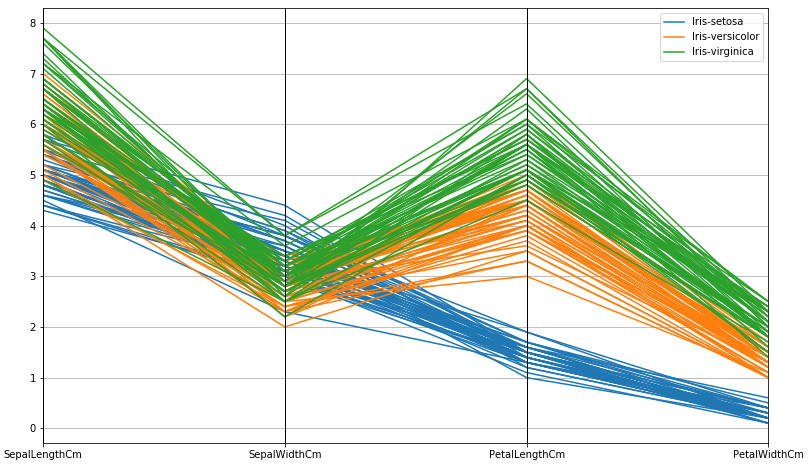
\includegraphics[width=0.7\textwidth]{iris-parallel.png}
 \caption{Parallel coordinates for the Iris dataset.}
 \label{fig:iris-parallel}
\end{figure}

\begin{figure}[ht]
 \centering
 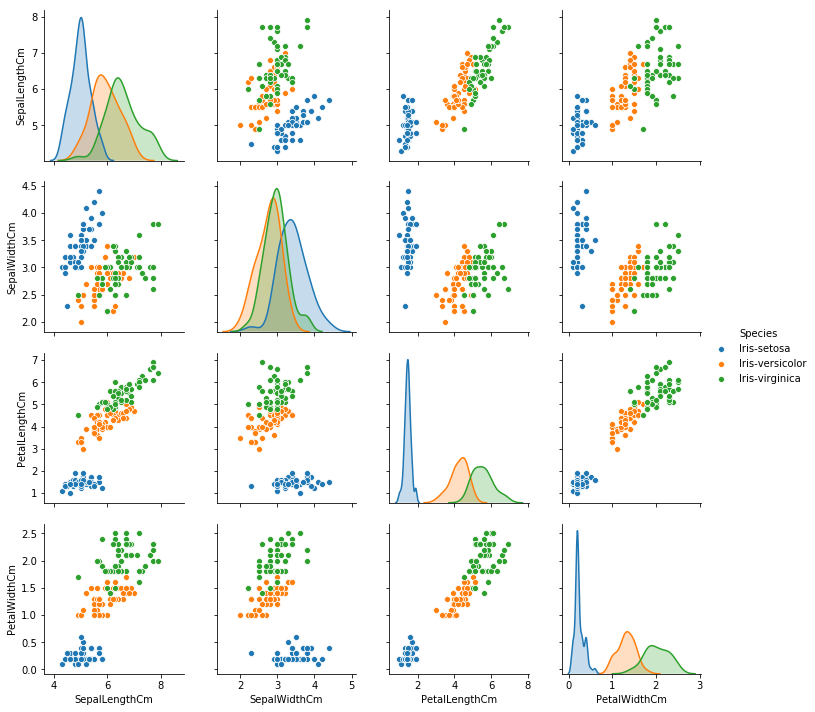
\includegraphics[width=0.9\textwidth]{iris-scatterplot.png}
 \caption{Scatter plot matrix for the Iris dataset.}
 \label{fig:iris-scatterplot}
\end{figure}

In the real-world, there are larger and more complex datasets than the Iris having hundreds of attributes and thousands or millions of items. For most of these cases, using the previous idioms is ineffective given the user cognition constraints for retaining many details, even when they are all shown at the same time, in addition to the screen size constraint. Next subsections describe two datasets considered relevant for this study and a possible exploratory analysis path supported by ML DR and Clustering algorithms.

\subsection{The FIFA 19 Complete Player Dataset}
\label{subsection1.1.1}

The FIFA dataset is currently one of the most popular datasets in Kaggle\footnote{https://www.kaggle.com/datasets (accessed on April 21th, 2019)}. It contains more than 18.000 player records of the popular video game, information representing the real state of players belonging to a wide variety of soccer clubs around the world. For each player there are 89 categorical and ordered attributes including age, nationality, overall scoring, potential, club, value, wage, preferred foot, international reputation, weak foot, skill moves, work rate, among many others. A possible user task could be to identify players with similar physical and game attributes to subsequently determine, for instance, the best conditions for training, trading options and match planning.

Figure \ref{fig:fifa-navio} summarizes this dataset by using Navio \cite{Guerra-Gomez2018Navio:Datasets} which is an interactive tool for exploring and navigating larger and high-dimensional datasets. More details about Navio are given in Section \ref{section4.3}. This is a good starting point for data understanding, nevertheless, it is not enough for fulfilling with the user task previously stated where attributes need to be aggregated in order to transversely identify similar players. 

\begin{figure}[ht]
 \centering
 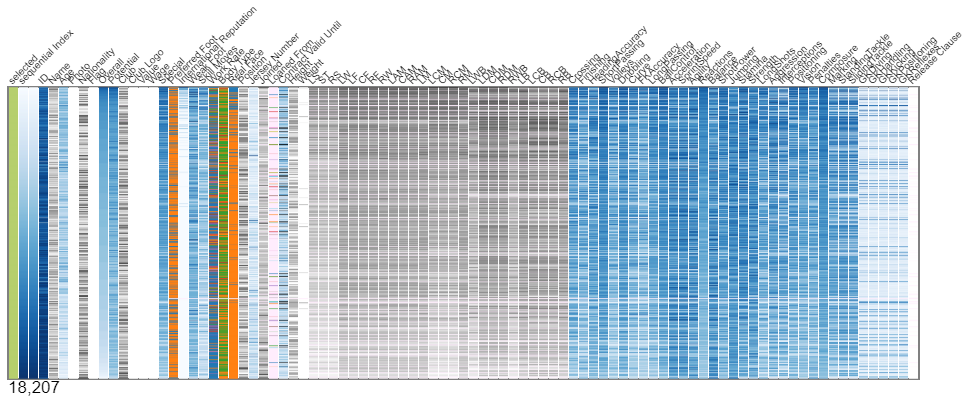
\includegraphics[width=0.9\textwidth]{fifa-navio.png}
 \caption{Visualization of the FIFA dataset in Navio.}
 \label{fig:fifa-navio}
\end{figure}

In this scenario is where ML can be useful. After validate data quality and transform attributes, a DR model is trained, for instance t-SNE, for producing an embedding that enables the identification of clusters of similar players. In addition, the position categorical attribute is used to encode the color in the embedding. The result is shown in Figure \ref{fig:fifa-tsne}. From this perspective, some analysis questions can be asked:

\begin{itemize}
\item Do clusters visually identified match with the position of the player? Do this match with other attribute in the dataset?
\item What characterize the players of the upper-left cluster and difference them from the players in the central cluster?
\item If goalkeepers (orange cluster) are excluded from the analysis, does the new t-SNE model produce the same three remaining clusters?
\item If physical attributes like height and weight are also excluded, is the player distribution in the embedding affected?  
\end{itemize}

\begin{figure}[ht]
 \centering
 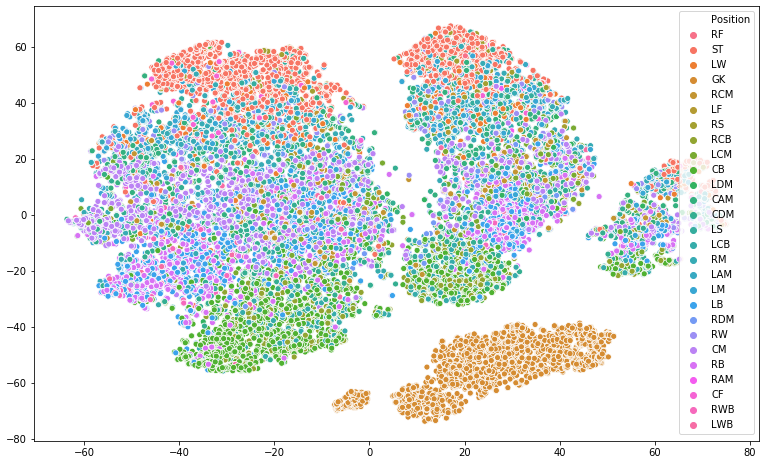
\includegraphics[width=0.7\textwidth]{fifa-tsne.png}
 \caption{DR embedding for the FIFA dataset using the t-SNE algorithm.}
 \label{fig:fifa-tsne}
\end{figure}

The first question could have a positive answer by performing model selection, which is addressed in Section \ref{section3.1}. Subsequent questions can be asked by additional experimentation where dataset is filtered or reduced and additional models are retrained in a iterative way. It is also required to be able for analyzing items in specific regions of the embedding. If the user is a ML-expert, they will not have problems to perform these analysis in the framework of their preference, otherwise, a tool for interact and interpret the model space and results is valuable. Some state of the art proposals are analyzed in Section \ref{section3.3}. Chapter \ref{chapter4} is focused on describing an improved proposal of a web interactive tool for answering these kind of EDA but also ML questions.

\subsection{The SALURBAL Dataset}
\label{subsection1.1.2}

SALURBAL is a five-year project aimed to study how urban environments and urban policies impact the health of city residents throughout Latin America \footnote{https://drexel.edu/lac/salurbal/overview/ (accessed on April 22th, 2019)}. For this purpose, datasets of Latin American cities and sub-cities containing urban form, landscape, street design and transportation metrics has been collected to subsequently determine which patterns emerge as mechanism for supporting the decision-making by domain-experts in fields like transportation and urban health. The sub-cities dataset has 1.438 items and 83 attributes, where all attributes are sequential except for name of the sub-city, type, city, country, presence of BRT, subway and aerial tram being categorical. Patterns can be builded as clusters, where sub-cities in the same cluster have similar metrics. In this sense, public policies already successful in one sub-city could have high probability to have success in other sub-city belonging to the same cluster. 

Again, the Figure \ref{fig:salurbal-navio} summarizes this dataset by using Navio enabling user to derive important instances by sorting and filtering interactions as explained in  in Section \ref{section4.3}.

\begin{figure}[ht]
 \centering
 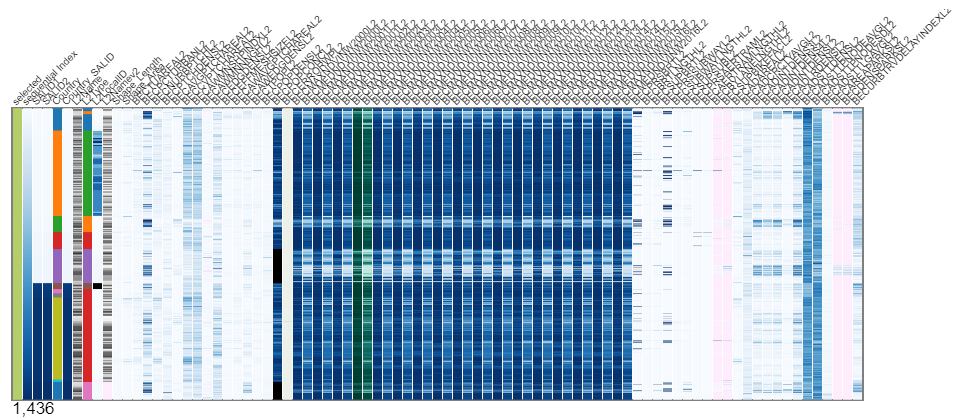
\includegraphics[width=0.9\textwidth]{salurbal-navio.png}
 \caption{Visualization of the SALURBAL dataset in Navio.}
 \label{fig:salurbal-navio}
\end{figure}

After validate data quality and transform attributes, a K-Means model is trained for producing groups of similar sub-cities that can be analyzed more easily. The model produces a cluster membership for each instance and a set of centroids but not much explanations about how these have been built. An alternative for gaining understanding is to observe the distribution of the original-space attributes, but since there are many of them, using t-SNE for visualizing the cluster distribution and validating their separability or overlapping is a reasonable choice. The result is shown in Figure \ref{fig:salurbal-kmeans-tsne}. Nevertheless, similar to the FIFA dataset, important questions need to be addressed: 

% Enfocar más a negocio
\begin{itemize}
\item Do the clusters of similar sub-cities match with the 2-dimensional distribution from the DR embedding?
\item What characterize the sub-cities of the blue cluster and difference them from the sub-cities in the red cluster?
\item Why the green cluster have only two sub-cities? Do they correspond to outliers having to be removed for the analysis? Does 4 clusters not represent a convenient data grouping?
\item These models are obtained including all sub-cities metrics for training. Would more make sense if models for Clustering and DR are trained by groups of attributes like urban landscape and street design?
\end{itemize}

\begin{figure}[ht]
 \centering
 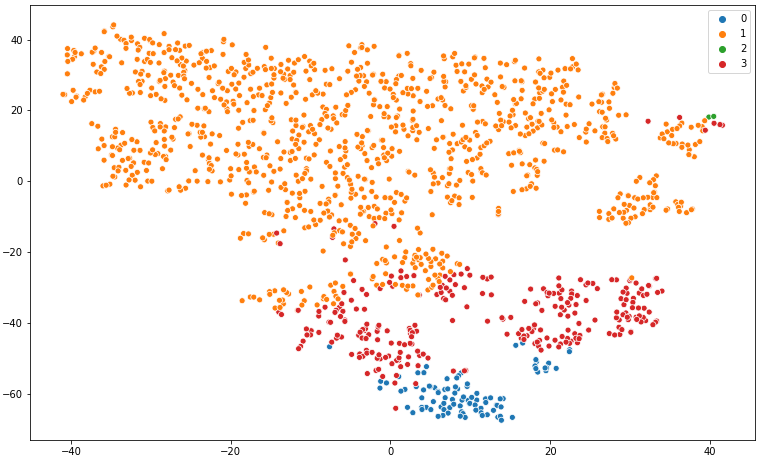
\includegraphics[width=0.7\textwidth]{salurbal-kmeans-tsne.png}
 \caption{DR embedding + Clustering for the SALURBAL dataset using the t-SNE and K-Means algorithms.}
 \label{fig:salurbal-kmeans-tsne}
\end{figure}

As stated in previous subsection, Chapters \ref{chapter3} and \ref{chapter4} are focused on describing some state of the art tools and an improved proposal of web interactive tool for answering these questions. 

\section{Document Structure} %Section - 1.2 
\label{section1.2}

This document is organized as follows: Chapter \ref{chapter2} shows the state of the art analysis for the Interactive ML and Interpretable ML sub-fields and the first contribution in terms of a set of guidelines for designing better and more user-centric ML systems. Chapter \ref{chapter3} describes some traditional DR and Clustering algorithms from a practical perspective and discuss the current advances for interact and interpret them in VA contexts. Chapter \ref{chapter4} presents the web interactive tool for exploring high-dimensional tabular data supported by t-SNE and K-Means. Chapter \ref{chapter5} evidences the results of the tool evaluation based on two real-world case studies. Finally, Chapter \ref{chapter6} concludes the work and presents the challenges and opportunities for the future.